%You should edit TheoryOfComputation-lecture00.tex, not this file!
\usepackage{fullpage}
\usepackage{color}
\usepackage{graphicx}
\usepackage{epsfig}
\usepackage{amsthm}
\usepackage{latexsym}
\usepackage{amssymb}
\usepackage{amsmath}
\usepackage{algorithmicx,algorithm}
\usepackage[noend]{algpseudocode}
\usepackage{verbatim}
\usepackage{mathrsfs}
%\usepackage{eso-pic}
\usepackage{unicode-math}
%\setmathfont{XITS Math}
\usepackage{xepersian}
\settextfont{XBZar}
%\setdigitfont{ParsiDigits}
%\defpersianfont\outline[Scale=1]{XBZar}


\newcommand{\newfontobj}[2]{
  \newcommand{#1}[1]{
    \expandafter\def\csname##1\endcsname{{#2 ##1}}}}

\newfontobj{\class}{\rm} % Typeset Classes in roman font

% Some standard classes (use in only mathmode)
% Usage example: $\P \subseteq \NP$ and we believe that $\NP$ is not 
%  equal to $\P$.


\class{PSPACE}	
\class{L}
\class{BPL}
\class{RL}
\class{NC}
\class{ZPL}
\class{NPSPACE}	
\class{ASPACE}	
\class{NL}
\class{EXP}
\class{NEXP}
\class{coNEXP}
\class{NE}
\class{E}
\class{AM}		
\class{MA}
\class{NP}
\class{DNP}
\class{UP}
\class{P}
\class{RP}
\class{BPP}
\class{ZPP}
\class{EXPSPACE}
\class{coNP}
\class{coRP}
\class{coAM}
\class{PH}
\class{IP}
\class{PCP}
\class{MIP}

% operator classes.
\class{BP}

% these commands should be used in math mode - $ $
\newcommand{\SHARPP}{{\#\rm{P}}}
\newcommand{\PARITYP}{{\oplus\rm{P}}}

% math operators...
\DeclareMathOperator{\poly}{poly}
\DeclareMathOperator{\Majority}{Majority}
\DeclareMathOperator{\quasipoly}{quasi-poly}
\DeclareMathOperator{\polylog}{poly-log}
\DeclareMathOperator{\superpoly}{super-poly}
\DeclareMathOperator{\DTISP}{DTISP}
\DeclareMathOperator{\DSPACE}{DSPACE}
\DeclareMathOperator{\DTIME}{DTIME}
\DeclareMathOperator{\NSPACE}{NSPACE}
\DeclareMathOperator{\NTIME}{NTIME}
\DeclareMathOperator{\BPTIME}{BPTIME}
\DeclareMathOperator{\RTIME}{RTIME}
\DeclareMathOperator{\ZPTIME}{ZPTIME}
\DeclareMathOperator{\BPSPACE}{BPSPACE}
\DeclareMathOperator{\RSPACE}{RSPACE}
\DeclareMathOperator{\ZPSPACE}{ZPSPACE}


% Complexity class
\newcommand{\CC}{\mathcal{C}}

%------------------------ Algorithm ------------------------------------

\newenvironment{الگوریتم}[1]
{\bigskip\bigskip\begin{algorithm}\caption{#1} \label{الگوریتم: #1}\vspace{0.5em}\begin{algorithmic}[1]}
		{\end{algorithmic}\vspace{0.5em}\end{algorithm}\bigskip}


\renewcommand{\algorithmicfor}{{به ازای}}
\renewcommand{\algorithmicwhile}{{تا وقتی}}
\renewcommand{\algorithmicdo}{\hspace{-.2em}:}
\renewcommand{\algorithmicif}{{اگر}}
\renewcommand{\algorithmicthen}{\hspace{-.2em}:}
\renewcommand{\algorithmicelse}{{در غیر این صورت:}}
%\renewcommand{\algorithmicelsif}{{در غیر این صورت اگر: }}
\renewcommand{\algorithmicreturn}{{برگردان}}
\renewcommand{\algorithmiccomment}[1]{$\triangleleft$ \emph{#1}}
\renewcommand{\algorithmicrequire}{\textbf{ورودی:}}
\renewcommand{\algorithmicensure}{\textbf{خروجی:}}

\newcommand{\اگر}{\If}
\newcommand{\وگرنه}{\Else}
\newcommand{\وگر}{\ElsIf}
%\newcommand{\پایان‌اگر}{\EndIf}
\newcommand{\بهه}{\For}
%\newcommand{\پایان‌به‌ازای}{\EndFor}
\newcommand{\تاوقتی}{\While}
%\newcommand{\پایان‌تاوقتی}{\EndWhile}
\newcommand{\دستور}{\State}
\newcommand{\دستورک}{\Statex}
\newcommand{\توضیحات}{\Comment}
\newcommand{\برگردان}{\Return}
\newcommand{\ورودی}{\Require}
\newcommand{\خروجی}{\Ensure}



%---------------------------------------------------------------------

% \lecture{number}{date}{title}{scribe}
\newcommand{\lecture}[2]{
\noindent
\fbox{
\begin{minipage}{6.2in}
 {\bf بازیابی پیشرفته‌ی اطلاعات}  \hfill 	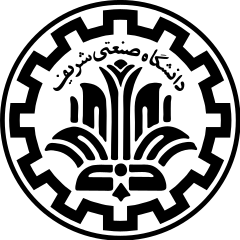
\includegraphics[scale=0.08]{Sharif.png}\hfill  نیم‌سال اول ۱۳۹۹-۱۳۹۸
  \begin{center}
    {\Large گزارش فاز #1 پروژه} \\[3mm]
  \end{center}
مدرس: دکتر بیگی\hfill اعضای گروه: #2
\end{minipage}
}
\bigskip

\bigskip
}
% \homework{number}{date}
\newcommand{\homework}[2]{
\noindent
\fbox{
\begin{minipage}{6.2in}
  {\bf CS 810: Complexity Theory} \hfill #2
  \begin{center}
    {\Large Homework #1} \\[3mm]
  \end{center}
Instructor: Dieter van Melkebeek \hfill TA: Jeff Kinne
\end{minipage}
}
\bigskip

\bigskip
}

% add DRAFT to your document %
\newcommand{\draft}[0]{
\begin{center}
	{\bf \LARGE {\sc نسخه اولیه} }
\end{center}
}

% example environment
\newenvironment{example}
{\smallskip \noindent \emph{مثال:}}
{\hfill $\boxtimes$ \smallskip}

% some theorem environments
\newtheorem{theorem}{قضیه}
\newtheorem{conjecture}[theorem]{حدس}
\newtheorem{proposition}{گزاره}
\newtheorem{claim}{ادعا}
\newtheorem{lemma}{لم}
\newtheorem{corollary}{نتیجه}
\newtheorem{definition}{تعریف} % Use this for non-trivial definitions.

% currently not used %
\newtheorem{exercise}{تمرین}
\newtheoremstyle{example}{\topsep}{\topsep}%
     {\normalfont \small}   % Body font
     {}    % Indent amount (empty = no indent, \parindent = para indent)
     {\bfseries}     % Thm head font
     {}%           Punctuation after thm head
     {\topsep}%     Space after thm head
     {}%         Thm head spec    \theoremstyle{example}
\theoremstyle{example}
%\newtheorem{example}{Example}

